\documentclass{article}
\usepackage[landscape]{geometry}
\usepackage[utf8]{inputenc}
\usepackage{tikz}
\usetikzlibrary{mindmap,backgrounds}
\pagestyle{empty}
\usepackage[T1]{fontenc}
\usepackage[utf8]{inputenc}
%lmodern	lmss
\usepackage{helvet}

\begin{document}
\pagestyle{empty}


{\fontfamily{hvt}
\centering
\begin{figure}
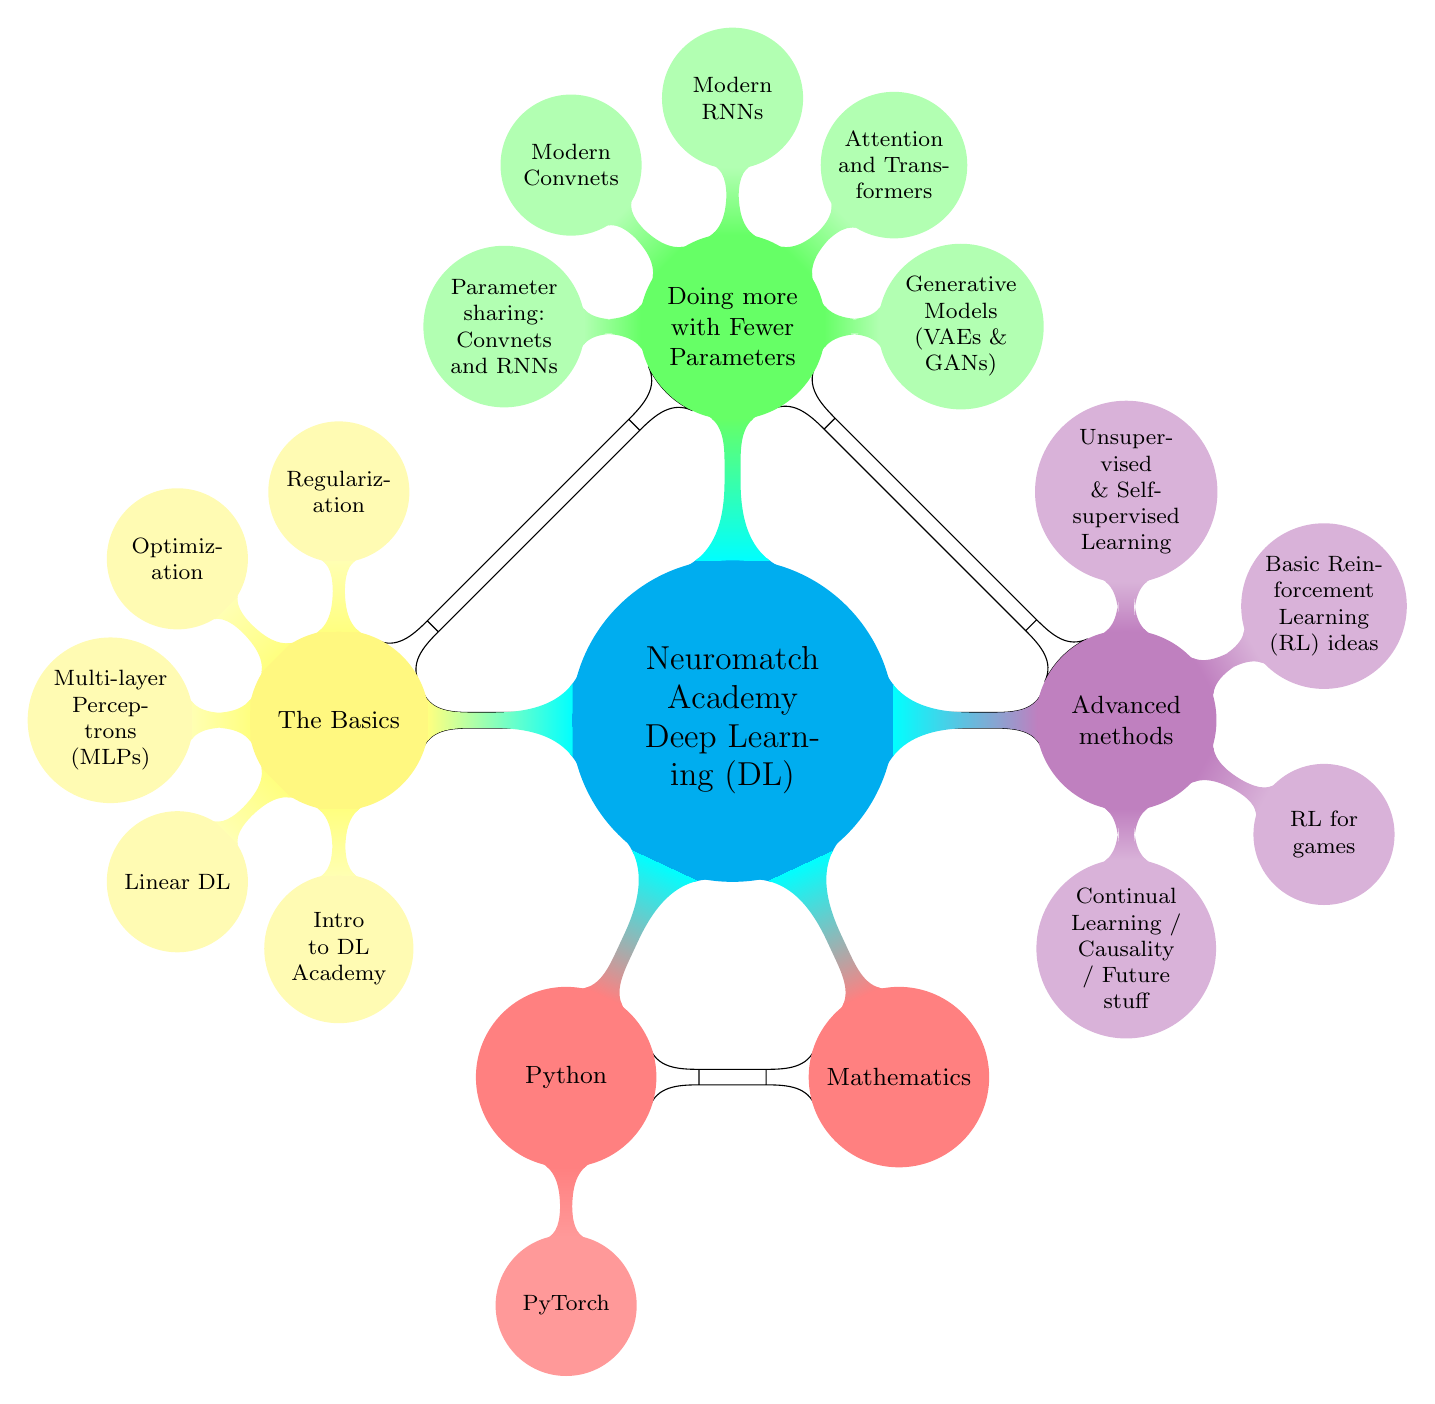
\begin{tikzpicture}




  
  \path[mindmap,concept color=cyan,text=black]
    node[concept,concept color=cyan!100](pde) {Neuromatch Academy \\ Deep Learning (DL)} 
    child[grow=245,concept color=red!50] { node[concept](Pyth) {Python} 
    child[grow=270, concept color=red!40] {
      node[concept](PyTor) {PyTorch}
    }
    }   
    child[grow=295,concept color=red!50]{node[concept] (Math){ Mathematics}    
    }
        % THE BASICS
             child[grow=180,concept color=yellow!50]{node[concept] (TheBasics){The Basics}
      % ModTy
      child[grow=270,concept color=yellow!30]{node[concept] (IntroDL){Intro to DL Academy}    }
      child[grow=225,concept color=yellow!30]{node[concept] (DLLinear){Linear DL}}
      child[grow=180,concept color=yellow!30]{node[concept] (MLP){Multi-layer Perceptrons (MLPs) }}
      child[grow=135,concept color=yellow!30]{node[concept] (Opt){Optimiz-\\ ation}}
      child[grow=90,concept color=yellow!30]{node[concept] (Reg){Regulariz-\\ ation}}
    }
    % Doing more with Fewer Parameters
       child[grow=90,concept color=green!60]{node[concept] (DmwFP){Doing more with Fewer Parameters}
   child [grow=180,concept color=green!30]
    {node [concept] (ParamShar) {Parameter sharing: Convnets and RNNs}
    }
    child [grow=135,concept color=green!30]
    {node [concept] (ModConv) {Modern Convnets}
    }
     child [grow=90,concept color=green!30]
    {node [concept] (ModRNN) {Modern RNNs}
    }
       child [grow=45,concept color=green!30]
    {node [concept] (Att&Trans) {Attention and Transformers}
    }
           child [grow=0,concept color=green!30]
    {node [concept] (GenMod) {Generative Models (VAEs \& GANs)}
    }
   }
     % Advanced methods
     child[grow=0,concept color=violet!50]{node[concept] (AdvMeth){ Advanced methods}
   child[grow=90,concept color=violet!30]{node[concept] (Unsup){Unsuper- \\ vised \& Self-supervised Learning }    }
 child[grow=30,concept color=violet!30]{node[concept] (BasRL){Basic Reinforcement Learning (RL) ideas}
   }
   child[grow=-30,concept color=violet!30]{node[concept] (RLgames){RL for games}
   }
    child[grow=-90,concept color=violet!30]{node[concept] (Con){Continual Learning / Causality / Future stuff}
   }
    };

   \begin{pgfonlayer}{background}
    \draw [circle connection bar]
      (TheBasics) edge (DmwFP)
      (DmwFP) edge (AdvMeth)
      (TheBasics) edge (AdvMeth) 
      (Pyth) edge (Math)
      ;
  \end{pgfonlayer}
\end{tikzpicture}

\end{figure}
}
\end{document}

